% !TeX root = 系统动力学建模与仿真笔记.tex

\section{运动学基础}
\subsection{简单转动}

由方向余弦矩阵的性质八即性质~\ref{prop:dcm-eigenvalue}，可以得出欧拉旋转定理（\textit{Euler's Rotation Theorem}）。

\begin{theorem}[欧拉旋转定理]\label{thm:euler-rotation}
	任意两个坐标系 $i$ 和 $j$ 之间的方向余弦矩阵 $\boldsymbol{A}_{ij}$ 都有一个实特征值 1，即存在一个实数形式的特征向量 $\boldsymbol{r}$，该特征向量满足 $\boldsymbol{r}=\boldsymbol{A}_{ij}\boldsymbol{r}$。该性质表明两坐标间的任意相对转动都可以通过一次定轴（简单）转动来完成，且转轴方向不变。

	即任意相对转动等价于一次定轴转动。
\end{theorem}

\begin{figure}[h]
	\centering
	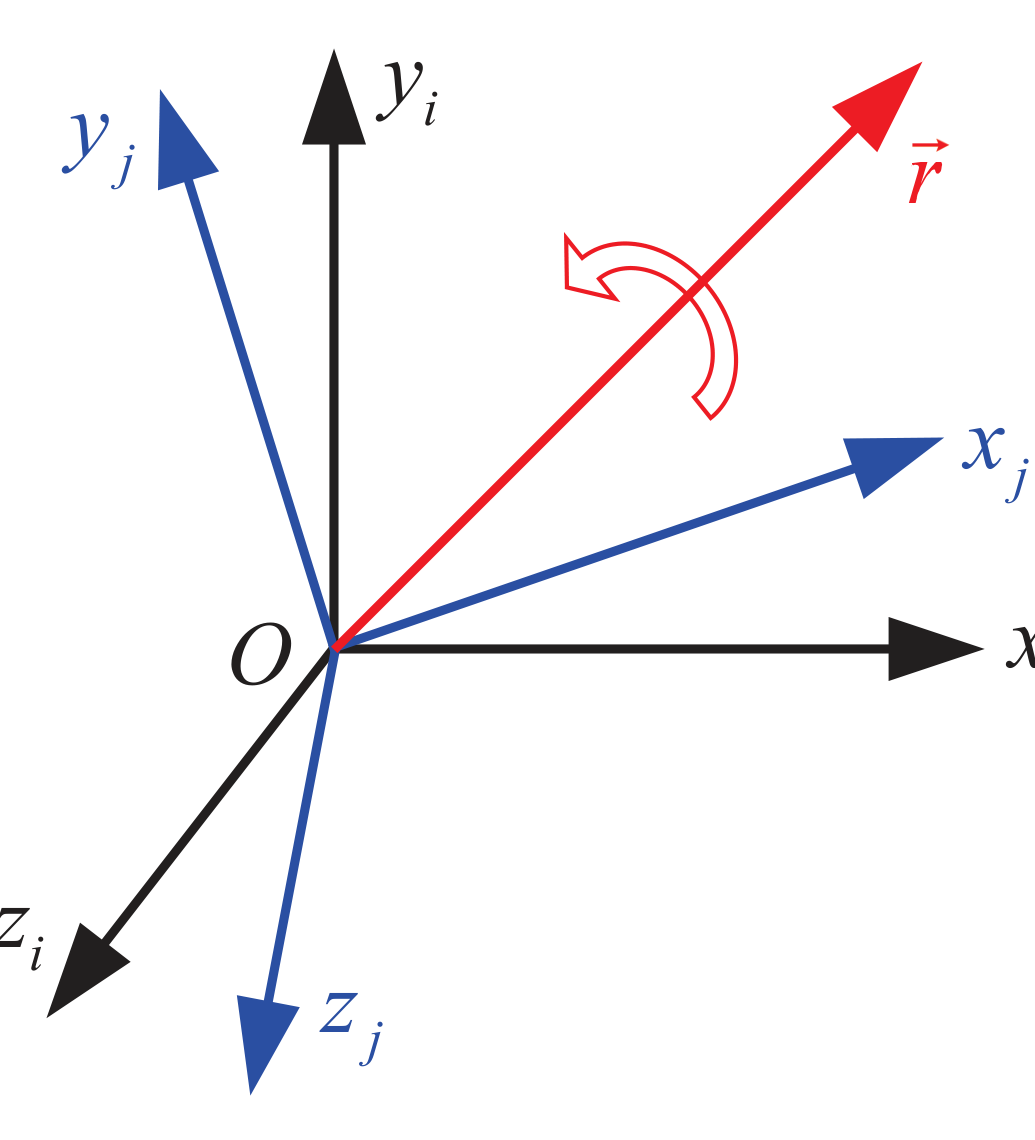
\includegraphics[width=0.4\linewidth]{Figure/两坐标系间的相对转动.png}
	\caption{简单旋转}
	\label{fig:简单旋转}
\end{figure}

两坐标系的相对方位与转轴单位矢量 $\vec{n}$ 和转角 $\theta$ 的关系是什么？下面通过简单转动来讨论。

\begin{figure}[H]
	\centering
	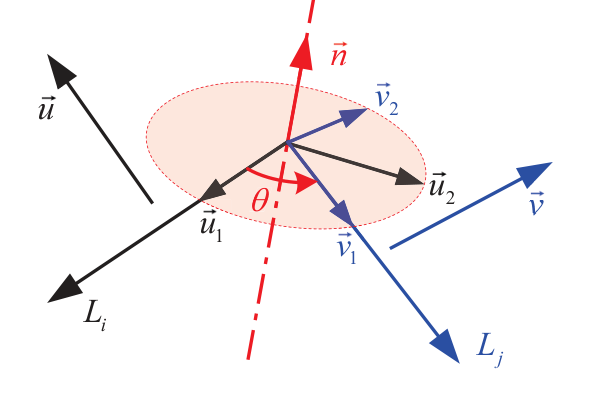
\includegraphics[width=0.7\linewidth]{Figure/任意三维矢量的定点简单转动}
	\caption{任意三维矢量的定点简单转动}
	\label{fig:任意三维矢量的定点简单转动}
\end{figure}

矢量 $\vec{u}$ 绕转轴 $L$（单位矢量 $\vec{n}$）转动 $\theta$ 角后变为 $\vec{v}$，图中 $\vec{u}_1$、$\vec{v}_1$ 为平行于转轴的分量，$\vec{u}_2$、$\vec{v}_2$ 为垂直于转轴的分量，$L_i$、$L_j$ 为参考直线。

\begin{theorem}[矢量定点转动公式]\label{thm:vector-rotation}
	矢量 $\vec{u}$ 绕单位矢量 $\vec{n}$ 所确定的轴转动角度 $\theta$ 后得到的矢量 $\vec{v}$ 为
	$$
	\vec{v}=\cos\theta\,\vec{u}+\sin\theta\,\vec{n}\times\vec{u}+(1-\cos\theta)\,\vec{n}\,(\vec{n}\cdot\vec{u}).
	$$
\end{theorem}

\begin{proof}
	将 $\vec{u}$ 分解为平行于转轴 $\vec{n}$ 的分量 $\vec{u}_{\parallel}$ 和垂直于转轴的分量 $\vec{u}_{\perp}$：
	$$
	\vec{u}_{\parallel}=(\vec{n}\cdot\vec{u})\,\vec{n}, \qquad
	\vec{u}_{\perp}=\vec{u}-\vec{u}_{\parallel}=\vec{u}-(\vec{n}\cdot\vec{u})\,\vec{n}.
	$$

	转动过程中，平行分量不变：$\vec{v}_{\parallel}=\vec{u}_{\parallel}$。

	垂直分量在垂直于 $\vec{n}$ 的平面内旋转 $\theta$ 角。设 $\vec{w}=\vec{n}\times\vec{u}$，由于 $\vec{n}$ 为单位矢量且 $\vec{u}_{\perp}\perp\vec{n}$，有
	$$
	|\vec{w}|=|\vec{n}|\,|\vec{u}_{\perp}|\sin\frac{\pi}{2}=|\vec{u}_{\perp}|, \quad \vec{w}\perp\vec{n}, \quad \vec{w}\perp\vec{u}_{\perp}.
	$$
	因此 $\vec{u}_{\perp}$ 与 $\vec{w}$ 构成垂直于 $\vec{n}$ 的平面内的一组正交基，$\vec{u}_{\perp}$ 旋转 $\theta$ 角后的结果为
	$$
	\vec{v}_{\perp}=\cos\theta\,\vec{u}_{\perp}+\sin\theta\,\vec{w}
	=\cos\theta\,\vec{u}_{\perp}+\sin\theta\,\vec{n}\times\vec{u}.
	$$

	叠加两个分量，得
	$$
	\vec{v}=\vec{v}_{\parallel}+\vec{v}_{\perp}
	=(\vec{n}\cdot\vec{u})\,\vec{n}+\cos\theta\,\vec{u}_{\perp}+\sin\theta\,\vec{n}\times\vec{u}.
	$$
	将 $\vec{u}_{\perp}=\vec{u}-(\vec{n}\cdot\vec{u})\,\vec{n}$ 代入：
	$$
	\vec{v}=(\vec{n}\cdot\vec{u})\,\vec{n}+\cos\theta\left[\vec{u}-(\vec{n}\cdot\vec{u})\,\vec{n}\right]+\sin\theta\,\vec{n}\times\vec{u},
	$$
	整理即得
	$$
	\vec{v}=\cos\theta\,\vec{u}+\sin\theta\,\vec{n}\times\vec{u}+(1-\cos\theta)\,\vec{n}\,(\vec{n}\cdot\vec{u}).
	$$
\end{proof}

上述等式两端分别向 $j$ 系和 $i$ 系投影可得
$$
\vec{e}_j^{\mathrm{T}}\boldsymbol{v}_j
=\vec{e}_i^{\mathrm{T}}\boldsymbol{u}_i\cos\theta
+\vec{e}_i^{\mathrm{T}}\tilde{\boldsymbol{n}}_i\boldsymbol{u}_i\sin\theta
+\vec{e}_i^{\mathrm{T}}\boldsymbol{n}_i\boldsymbol{n}_i^{\mathrm{T}}\boldsymbol{u}_i(1-\cos\theta)
=\vec{e}_i^{\mathrm{T}}\left[\boldsymbol{I}_3\cos\theta+\tilde{\boldsymbol{n}}_i\sin\theta+\boldsymbol{n}_i\boldsymbol{n}_i^{\mathrm{T}}(1-\cos\theta)\right]\boldsymbol{u}_i.
$$

注意到
$$
\vec{e}_j^{\mathrm{T}}=(\boldsymbol{A}_{ji}\vec{e}_i)^{\mathrm{T}}=\vec{e}_i^{\mathrm{T}}\boldsymbol{A}_{ji}^{\mathrm{T}}=\vec{e}_i^{\mathrm{T}}\boldsymbol{A}_{ij},\qquad\boldsymbol{v}_j=\boldsymbol{u}_i,\qquad\boldsymbol{n}_j=\boldsymbol{n}_i=:\boldsymbol{n},
$$

将其代入三维矢量定点简单转动表达式可得
$$
\vec{e}_i^{\mathrm{T}}\boldsymbol{A}_{ij}\boldsymbol{u}_i=\vec{e}_i^{\mathrm{T}}\left[\boldsymbol{I}_3\cos\theta+\tilde{\boldsymbol{n}}\sin\theta+\boldsymbol{n}\boldsymbol{n}^{\mathrm{T}}(1-\cos\theta)\right]\boldsymbol{u}_i.
$$

移项后整理可得
$$
\vec{e}_i^{\mathrm{T}}\left\{\boldsymbol{A}_{ij}-\left[\boldsymbol{I}_3\cos\theta+\tilde{\boldsymbol{n}}\sin\theta+\boldsymbol{n}\boldsymbol{n}^{\mathrm{T}}(1-\cos\theta)\right]\right\}\boldsymbol{u}_i=\vec{0}.
$$

由上式可得
$$
\left\{\boldsymbol{A}_{ij}-\left[\boldsymbol{I}_3\cos\theta+\tilde{\boldsymbol{n}}\sin\theta+\boldsymbol{n}\boldsymbol{n}^{\mathrm{T}}(1-\cos\theta)\right]\right\}\boldsymbol{u}_i=\boldsymbol{0}.
$$

进一步，由 $\boldsymbol{u}_i$ 的任意性可得
$$
\boldsymbol{A}_{ij}-\left[\boldsymbol{I}_3\cos\theta+\tilde{\boldsymbol{n}}\sin\theta+\boldsymbol{n}\boldsymbol{n}^{\mathrm{T}}(1-\cos\theta)\right]=\boldsymbol{O}_{3\times3}.
$$

由此可得方向余弦矩阵与转轴转角的关系式，即

\begin{theorem}[罗德里格斯旋转公式]\label{thm:rodrigues}
	方向余弦矩阵与转轴单位矢量 $\vec{n}$ 及转角 $\theta$ 的关系为
	$$
	\boldsymbol{A}_{ij}=\boldsymbol{I}_3\cos\theta+\tilde{\boldsymbol{n}}\sin\theta+\boldsymbol{n}\boldsymbol{n}^{\mathrm{T}}(1-\cos\theta)=\boldsymbol{I}_3+\tilde{\boldsymbol{n}}\sin\theta+\tilde{\boldsymbol{n}}^2(1-\cos\theta).
	$$
\end{theorem}

\begin{proof}
	由矢量定点转动公式（定理~\ref{thm:vector-rotation}），对任意矢量 $\vec{u}$ 有
	$$
	\vec{v}=\cos\theta\,\vec{u}+\sin\theta\,\vec{n}\times\vec{u}+(1-\cos\theta)\,\vec{n}\,(\vec{n}\cdot\vec{u}).
	$$
	将等式两端向 $i$ 系投影。利用叉积的矩阵表示 $\vec{n}\times\vec{u}\leftrightarrow\tilde{\boldsymbol{n}}\boldsymbol{u}$ 以及点积的矩阵表示 $\vec{n}\cdot\vec{u}\leftrightarrow\boldsymbol{n}^{\mathrm{T}}\boldsymbol{u}$，可得
	$$
	\boldsymbol{v}_i=\cos\theta\,\boldsymbol{u}_i+\sin\theta\,\tilde{\boldsymbol{n}}\boldsymbol{u}_i+(1-\cos\theta)\,\boldsymbol{n}\boldsymbol{n}^{\mathrm{T}}\boldsymbol{u}_i.
	$$
	另一方面，由性质~\ref{prop:dcm-transform} 知 $\boldsymbol{v}_j=\boldsymbol{A}_{ij}^{\mathrm{T}}\boldsymbol{v}_i$。因 $\boldsymbol{v}_j=\boldsymbol{u}_i$（转动不改变矢量本身，只改变其在不同坐标系中的投影），故
	$$
	\boldsymbol{A}_{ij}^{\mathrm{T}}\boldsymbol{v}_i=\boldsymbol{u}_i \quad\Longrightarrow\quad \boldsymbol{v}_i=\boldsymbol{A}_{ij}\boldsymbol{u}_i.
	$$
	代入上式得
	$$
	\boldsymbol{A}_{ij}\boldsymbol{u}_i=\left[\boldsymbol{I}_3\cos\theta+\tilde{\boldsymbol{n}}\sin\theta+\boldsymbol{n}\boldsymbol{n}^{\mathrm{T}}(1-\cos\theta)\right]\boldsymbol{u}_i.
	$$
	由 $\boldsymbol{u}_i$ 的任意性即得
	$$
	\boldsymbol{A}_{ij}=\boldsymbol{I}_3\cos\theta+\tilde{\boldsymbol{n}}\sin\theta+\boldsymbol{n}\boldsymbol{n}^{\mathrm{T}}(1-\cos\theta).
	$$
	又由性质~\ref{prop:dcm-cofactor} 可知 $\boldsymbol{n}\boldsymbol{n}^{\mathrm{T}}=\tilde{\boldsymbol{n}}^2+\boldsymbol{I}_3$ 不成立的一般情形下，注意到 $\tilde{\boldsymbol{n}}^2=\boldsymbol{n}\boldsymbol{n}^{\mathrm{T}}-\boldsymbol{I}_3$（叉乘矩阵性质），故 $\boldsymbol{n}\boldsymbol{n}^{\mathrm{T}}=\tilde{\boldsymbol{n}}^2+\boldsymbol{I}_3$，代入得
	$$
	\boldsymbol{A}_{ij}=\boldsymbol{I}_3+\tilde{\boldsymbol{n}}\sin\theta+\tilde{\boldsymbol{n}}^2(1-\cos\theta).
	$$
\end{proof}

罗德里格斯旋转公式的特殊形式：

\begin{property}[基本旋转矩阵]\label{prop:basic-rotation}
	当转轴分别沿三个坐标轴方向时，罗德里格斯旋转公式退化为基本旋转矩阵。

	转轴沿 $x$ 轴，即 $\boldsymbol{n}=[1\ 0\ 0]^{\mathrm{T}}$ 时，
	$$
	\boldsymbol{A}_x(\theta)=\begin{bmatrix}1&0&0\\0&\cos\theta&-\sin\theta\\0&\sin\theta&\cos\theta\end{bmatrix}.
	$$

	转轴沿 $y$ 轴，即 $\boldsymbol{n}=[0\ 1\ 0]^{\mathrm{T}}$ 时，
	$$
	\boldsymbol{A}_y(\theta)=\begin{bmatrix}\cos\theta&0&\sin\theta\\0&1&0\\-\sin\theta&0&\cos\theta\end{bmatrix}.
	$$

	转轴沿 $z$ 轴，即 $\boldsymbol{n}=[0\ 0\ 1]^{\mathrm{T}}$ 时，
	$$
	\boldsymbol{A}_z(\theta)=\begin{bmatrix}\cos\theta&-\sin\theta&0\\\sin\theta&\cos\theta&0\\0&0&1\end{bmatrix}.
	$$
\end{property}

\subsection{由方向余弦矩阵反求转轴和转角}
罗德里格斯旋转公式：
$$\begin{aligned}
	\boldsymbol{A}_{i j} & =\boldsymbol{I}_{3} \cos \theta+\tilde{\boldsymbol{n}} \sin \theta+\boldsymbol{n} \boldsymbol{n}^{\mathrm{T}}(1-\cos \theta) \\
	& =\left[\begin{array}{rrr}
		\cos \theta+n_{1} n_{1}(1-\cos \theta) & -n_{3} \sin \theta+n_{1} n_{2}(1-\cos \theta) & n_{2} \sin \theta+n_{1} n_{3}(1-\cos \theta) \\
		n_{3} \sin \theta+n_{2} n_{1}(1-\cos \theta) & \cos \theta+n_{2} n_{2}(1-\cos \theta) & -n_{1} \sin \theta+n_{2} n_{3}(1-\cos \theta) \\
		-n_{2} \sin \theta+n_{3} n_{1}(1-\cos \theta) & n_{1} \sin \theta+n_{3} n_{2}(1-\cos \theta) & \cos \theta+n_{3} n_{3}(1-\cos \theta)
	\end{array}\right] \\
	& =:\left[\begin{array}{lll}
		a_{11} & a_{12} & a_{13} \\
		a_{21} & a_{22} & a_{23} \\
		a_{31} & a_{32} & a_{33}
	\end{array}\right] .
\end{aligned}$$

由上式可知:$$\begin{aligned}
	\operatorname{tr} \boldsymbol{A} & =a_{11}+a_{12}+a_{33} \\
	& =3 \cos \theta+\left(n_{1}^{2}+n_{2}^{2}+n_{3}^{2}\right)(1-\cos \theta) \\
	& =2 \cos \theta+1,
\end{aligned}$$

以及反对称部分：

$$
\begin{cases}a_{32}-a_{23}=2n_1\sin\theta,\\a_{13}-a_{31}=2n_2\sin\theta,\\a_{21}-a_{12}=2n_3\sin\theta.\end{cases}
$$

于是由方向余弦矩阵反求转轴和转角：

$$
\begin{cases}\cos\theta=(\mathrm{tr}\,\boldsymbol{A}-1)/2,\\n_1\sin\theta=(a_{32}-a_{23})/2,\\n_2\sin\theta=(a_{13}-a_{31})/2,\\n_3\sin\theta=(a_{21}-a_{12})/2.\end{cases}
$$

若约定 $\theta\in[0,\pi]$，则分三种情形：

(1) 当 $|(\mathrm{tr}\,\boldsymbol{A}-1)/2-1|<\varepsilon$ 时，$\cos\theta\approx1$，$\sin\theta\approx0$，即 $\theta\approx0$，$\boldsymbol{A}\approx\boldsymbol{I}_3$，转轴 $\boldsymbol{n}$ 可为任意单位矢量列阵。

(2) 当 $|(\mathrm{tr}\,\boldsymbol{A}-1)/2+1|<\varepsilon$ 时，$\cos\theta\approx-1$，$\sin\theta\approx0$，即 $\theta\approx\pi$，$(\boldsymbol{A}+\boldsymbol{I})/2\approx\boldsymbol{n}\boldsymbol{n}^{\mathrm{T}}$，依此确定 $\boldsymbol{n}$ 的按模最大分量后即可求出完整的 $\boldsymbol{n}$。

(3) 当 $|(\mathrm{tr}\,\boldsymbol{A}-1)/2-1|>\varepsilon$ 且 $|(\mathrm{tr}\,\boldsymbol{A}-1)/2+1|>\varepsilon$ 时，

$$
\begin{cases}\theta=\mathrm{acos}\left((\mathrm{tr}\,\boldsymbol{A}-1)/2\right),\\n_1=(a_{32}-a_{23})/(2\sin\theta),\\n_2=(a_{13}-a_{31})/(2\sin\theta),\\n_3=(a_{21}-a_{12})/(2\sin\theta).\end{cases}
$$

\subsection{相对转动角速度}

上一小节研究了坐标系的转换关系，属于位置级的关系。本节将进一步讨论速度级的关系，引入相对转动角速度的概念。

\begin{figure}[H]
	\centering
	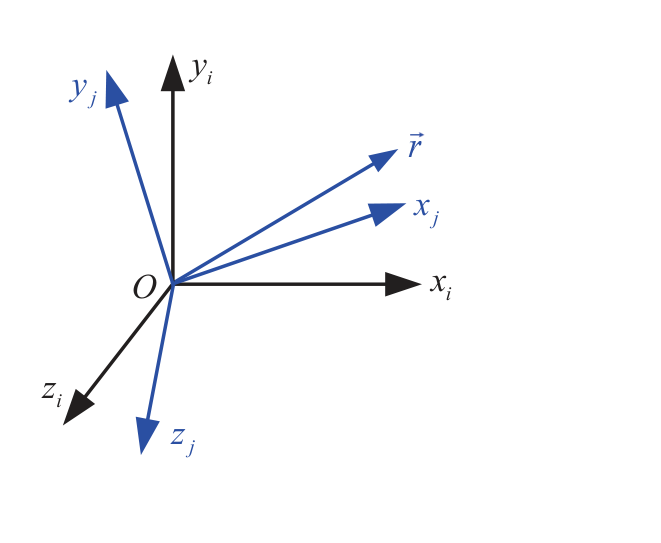
\includegraphics[width=0.7\linewidth]{Figure/固结在动系上的点的相对速度}
	\caption{固结在动系上的点}
	\label{fig:固结在动系上的点}
\end{figure}

\begin{definition}[方向余弦矩阵的时间变化率]\label{def:dcm-rate}
	设方向余弦矩阵 $\boldsymbol{A}_{ij}$ 随时间变化。由正交性 $\boldsymbol{A}_{ij}\boldsymbol{A}_{ij}^{\mathrm{T}}=\boldsymbol{I}_3$ 和 $\boldsymbol{A}_{ij}^{\mathrm{T}}\boldsymbol{A}_{ij}=\boldsymbol{I}_3$ 分别对时间求导，可知 $\dot{\boldsymbol{A}}_{ij}\boldsymbol{A}_{ij}^{\mathrm{T}}$ 和 $\boldsymbol{A}_{ij}^{\mathrm{T}}\dot{\boldsymbol{A}}_{ij}$ 均为反对称矩阵。定义
	$$
	\tilde{\boldsymbol{\omega}}_{ij|i}\triangleq\dot{\boldsymbol{A}}_{ij}\boldsymbol{A}_{ij}^{\mathrm{T}}, \qquad
	\tilde{\boldsymbol{\omega}}_{ij|j}\triangleq\boldsymbol{A}_{ij}^{\mathrm{T}}\dot{\boldsymbol{A}}_{ij},
	$$
	其中 $\boldsymbol{\omega}_{ij|i}$ 为 $j$ 系相对于 $i$ 系的相对转动角速度在 $i$ 系中的投影列阵，$\boldsymbol{\omega}_{ij|j}$ 为同一角速度在 $j$ 系中的投影列阵。
\end{definition}

\begin{proof}
	由 $\boldsymbol{A}_{ij}\boldsymbol{A}_{ij}^{\mathrm{T}}=\boldsymbol{I}_3$ 两边对时间求导：
	$$
	\boldsymbol{O}_3
	=\frac{\mathrm{d}}{\mathrm{d}t}\left(\boldsymbol{A}_{ij}\boldsymbol{A}_{ij}^{\mathrm{T}}\right)
	=\dot{\boldsymbol{A}}_{ij}\boldsymbol{A}_{ij}^{\mathrm{T}}+\boldsymbol{A}_{ij}\dot{\boldsymbol{A}}_{ij}^{\mathrm{T}}
	=\dot{\boldsymbol{A}}_{ij}\boldsymbol{A}_{ij}^{\mathrm{T}}+\left(\dot{\boldsymbol{A}}_{ij}\boldsymbol{A}_{ij}^{\mathrm{T}}\right)^{\mathrm{T}},
	$$
	故 $\dot{\boldsymbol{A}}_{ij}\boldsymbol{A}_{ij}^{\mathrm{T}}$ 为反对称矩阵。同理，由 $\boldsymbol{A}_{ij}^{\mathrm{T}}\boldsymbol{A}_{ij}=\boldsymbol{I}_3$ 求导可证 $\boldsymbol{A}_{ij}^{\mathrm{T}}\dot{\boldsymbol{A}}_{ij}$ 为反对称矩阵。
\end{proof}

由定义~\ref{def:dcm-rate} 可立即得到方向余弦矩阵时间变化率的两种等价表达：

\begin{property}[方向余弦矩阵的时间变化率]\label{prop:dcm-rate}
	方向余弦矩阵的时间导数满足
	$$
	\dot{\boldsymbol{A}}_{ij}=\tilde{\boldsymbol{\omega}}_{ij|i}\boldsymbol{A}_{ij}=\boldsymbol{A}_{ij}\tilde{\boldsymbol{\omega}}_{ij|j},
	$$
	且两个投影列阵通过方向余弦矩阵联系：
	$$
	\tilde{\boldsymbol{\omega}}_{ij|i}\boldsymbol{A}_{ij}=\boldsymbol{A}_{ij}\tilde{\boldsymbol{\omega}}_{ij|j}, \qquad
	\boldsymbol{\omega}_{ij|i}=\boldsymbol{A}_{ij}\boldsymbol{\omega}_{ij|j}.
	$$
	写成矢量形式为
	$$
	\vec{\omega}_{ij}=\vec{e}_i^{\mathrm{T}}\boldsymbol{\omega}_{ij|i}=\vec{e}_j^{\mathrm{T}}\boldsymbol{\omega}_{ij|j}.
	$$
\end{property}

\begin{proof}
	由 $\tilde{\boldsymbol{\omega}}_{ij|i}=\dot{\boldsymbol{A}}_{ij}\boldsymbol{A}_{ij}^{\mathrm{T}}$ 右乘 $\boldsymbol{A}_{ij}$ 即得 $\dot{\boldsymbol{A}}_{ij}=\tilde{\boldsymbol{\omega}}_{ij|i}\boldsymbol{A}_{ij}$；
	由 $\tilde{\boldsymbol{\omega}}_{ij|j}=\boldsymbol{A}_{ij}^{\mathrm{T}}\dot{\boldsymbol{A}}_{ij}$ 左乘 $\boldsymbol{A}_{ij}$ 即得 $\dot{\boldsymbol{A}}_{ij}=\boldsymbol{A}_{ij}\tilde{\boldsymbol{\omega}}_{ij|j}$。
	两式联立即得 $\tilde{\boldsymbol{\omega}}_{ij|i}\boldsymbol{A}_{ij}=\boldsymbol{A}_{ij}\tilde{\boldsymbol{\omega}}_{ij|j}$，再利用性质~\ref{prop:dcm-skew-transform} 即得投影列阵的变换关系。
\end{proof}

有了上述预备结论，下面讨论固结在动系上的点的相对速度。

\begin{theorem}[固结矢量的相对速度]\label{thm:relative-velocity}
	设矢量 $\vec{r}$ 固结在动系 $j$ 上，其在 $i$ 系中的投影列阵为 $\boldsymbol{r}_i=\boldsymbol{A}_{ij}\boldsymbol{r}_j$。由于 $\vec{r}$ 固结在 $j$ 系中，有 $\dot{\boldsymbol{r}}_j=\boldsymbol{0}$，则其相对速度为
	$$
	\dot{\boldsymbol{r}}_i=\tilde{\boldsymbol{\omega}}_{ij|i}\boldsymbol{A}_{ij}\boldsymbol{r}_j=\boldsymbol{A}_{ij}\tilde{\boldsymbol{\omega}}_{ij|j}\boldsymbol{r}_j.
	$$
	写成矢量形式为
	$$
	\vec{v}=\vec{\omega}_{ij}\times\vec{r},
	$$
	即固结在动系上的点的相对速度等于相对转动角速度与该矢量的叉积。
\end{theorem}

\begin{proof}
	对 $\boldsymbol{r}_i=\boldsymbol{A}_{ij}\boldsymbol{r}_j$ 两边对时间求导：
	$$
	\dot{\boldsymbol{r}}_i=\dot{\boldsymbol{A}}_{ij}\boldsymbol{r}_j+\boldsymbol{A}_{ij}\dot{\boldsymbol{r}}_j.
	$$
	因 $\vec{r}$ 固结在 $j$ 系中，故 $\dot{\boldsymbol{r}}_j=\boldsymbol{0}$，于是
	$$
	\dot{\boldsymbol{r}}_i=\dot{\boldsymbol{A}}_{ij}\boldsymbol{r}_j.
	$$
	将性质~\ref{prop:dcm-rate} 中 $\dot{\boldsymbol{A}}_{ij}$ 的两种表达代入，即得
	$$
	\dot{\boldsymbol{r}}_i=\tilde{\boldsymbol{\omega}}_{ij|i}\boldsymbol{A}_{ij}\boldsymbol{r}_j=\boldsymbol{A}_{ij}\tilde{\boldsymbol{\omega}}_{ij|j}\boldsymbol{r}_j.
	$$
	写成矢量形式，利用叉积的矩阵表示：
	$$
	\vec{v}=\vec{e}_i^{\mathrm{T}}\dot{\boldsymbol{r}}_i
	=\vec{e}_i^{\mathrm{T}}\tilde{\boldsymbol{\omega}}_{ij|i}\boldsymbol{A}_{ij}\boldsymbol{r}_j
	=\vec{e}_i^{\mathrm{T}}\tilde{\boldsymbol{\omega}}_{ij|i}\vec{e}_i^{\mathrm{T}}\cdot\vec{e}_j\boldsymbol{r}_j
	=\vec{\omega}_{ij}\times\vec{r}.
	$$
\end{proof}

\begin{figure}[H]
	\centering
	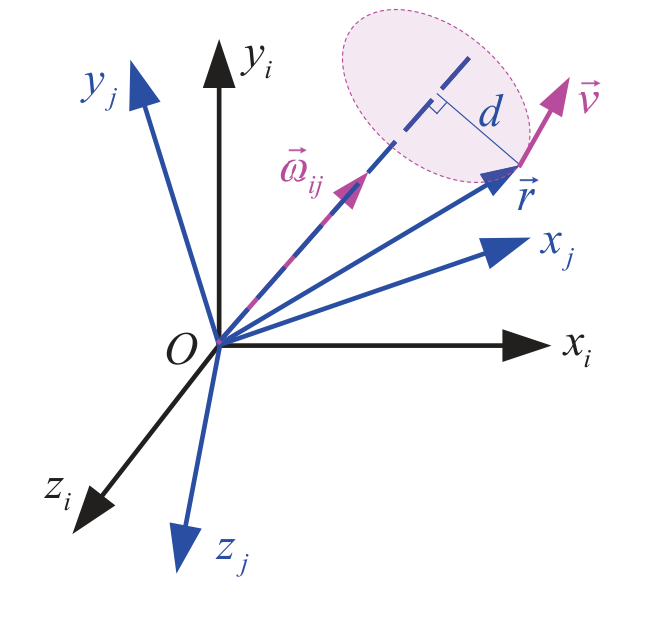
\includegraphics[width=0.7\linewidth]{Figure/固结在动系上的点的相对速度矢量}
	\caption{固结在动系上的点的相对速度矢量}
	\label{fig:固结在动系上的点的相对速度矢量}
\end{figure}

\begin{property}[相对速度的几何性质]\label{prop:relative-velocity-geometry}
	固结在动系上的点的相对速度 $\vec{v}=\vec{\omega}_{ij}\times\vec{r}$ 满足
	$$
	\vec{v}\perp\vec{\omega}_{ij}, \quad \vec{v}\perp\vec{r}, \quad
	|\vec{v}|=\left|\vec{\omega}_{ij}\right||\vec{r}|\sin\left\langle\vec{\omega}_{ij},\vec{r}\right\rangle=\left|\vec{\omega}_{ij}\right|d,
	$$
	其中 $d$ 为矢量 $\vec{r}$ 的末端到转轴的垂直距离。由此可知 $j$ 系相对于 $i$ 系作瞬时定轴转动，相对转动角速度为 $\vec{\omega}_{ij}$。
\end{property}
\begin{theorem}[科里奥利公式]
	科里奥利公式:
	$$\left.\frac{\mathrm{d} \vec{r}}{\mathrm{~d} t}\right|_{i}=\left.\frac{\mathrm{d} \vec{r}}{\mathrm{~d} t}\right|_{j}+\vec{\omega}_{i j} \times \vec{r}$$
\end{theorem}
\begin{proof}
	$$\begin{aligned}
		\dot{\boldsymbol{r}}_{i} & =\boldsymbol{A}_{i j} \dot{\boldsymbol{r}}_{j}+\dot{\boldsymbol{A}}_{i j} \boldsymbol{r}_{j} \\
		& =\boldsymbol{A}_{i j} \dot{\boldsymbol{r}}_{j}+\boldsymbol{A}_{i j} \tilde{\boldsymbol{\omega}}_{i j \mid j} \boldsymbol{r}_{j} . \\
		\overrightarrow{\boldsymbol{e}}_{i}^{\mathrm{T}} \dot{\boldsymbol{r}}_{i} & =\overrightarrow{\boldsymbol{e}}_{i}^{\mathrm{T}} \boldsymbol{A}_{i j} \dot{\boldsymbol{r}}_{j}+\overrightarrow{\boldsymbol{e}}_{i}^{\mathrm{T}} \boldsymbol{A}_{i j} \tilde{\boldsymbol{\omega}}_{i j \mid j} \boldsymbol{r}_{j} .
	\end{aligned}$$
\end{proof}

\begin{theorem}[角速度叠加定理]
	角速度叠加定理:
	$$\vec{\omega}_{i k}=\vec{\omega}_{i j}+\vec{\omega}_{j k}$$
\end{theorem}

\begin{proof}
	$$\begin{aligned}
		\vec{e}_{i} & =\boldsymbol{A}_{i j} \overrightarrow{\boldsymbol{e}}_{j}=\boldsymbol{A}_{i j} \boldsymbol{A}_{j k} \overrightarrow{\boldsymbol{e}}_{k}, \\
		\boldsymbol{A}_{i k} & =\overrightarrow{\boldsymbol{e}}_{i} \cdot \overrightarrow{\boldsymbol{e}}_{k}^{\mathrm{T}}=\boldsymbol{A}_{i j} \boldsymbol{A}_{j k}, \\
		\dot{A}_{i k} & =\dot{A}_{i j} \boldsymbol{A}_{j k}+\boldsymbol{A}_{i j} \dot{A}_{j k}, \\
		\boldsymbol{A}_{i k} \tilde{\boldsymbol{\omega}}_{i k \mid k} & =\boldsymbol{A}_{i j} \tilde{\boldsymbol{\omega}}_{i j \mid j} \boldsymbol{A}_{j k}+\boldsymbol{A}_{i j} \boldsymbol{A}_{j k} \tilde{\boldsymbol{\omega}}_{j k \mid k}, \\
		\tilde{\boldsymbol{\omega}}_{i k \mid i} & =\tilde{\boldsymbol{\omega}}_{i j \mid i}+\tilde{\boldsymbol{\omega}}_{j k \mid i}, \\
		\boldsymbol{\omega}_{i k \mid i} & =\boldsymbol{\omega}_{i j \mid i}+\boldsymbol{\omega}_{j k \mid i} .
	\end{aligned}$$
\end{proof}
\begin{figure}[H]
\centering
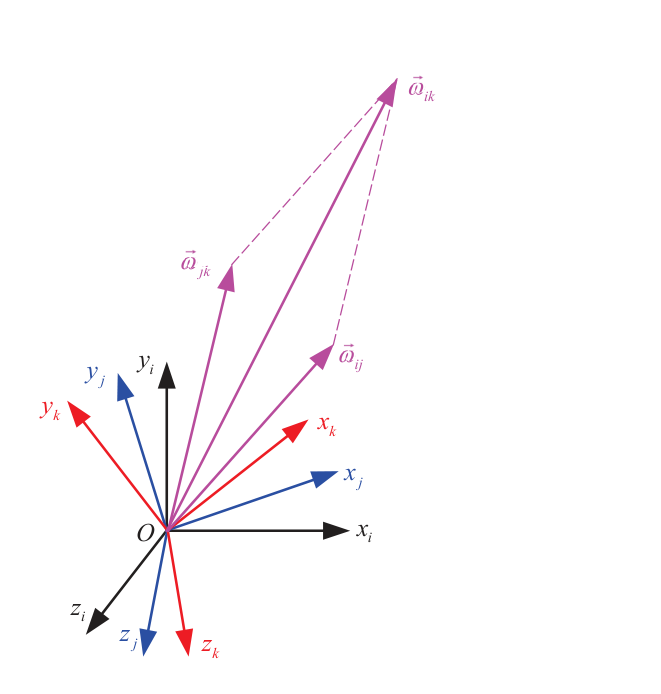
\includegraphics[width=0.7\linewidth]{Figure/角速度叠加定理}
\caption{角速度叠加定理}
\label{fig:角速度叠加定理}
\end{figure}
用转轴和转角表示的相对转动角速度矢量在动系中的投影列阵为

\begin{theorem}[角速度的转轴-转角表达]\label{thm:omega-n-theta}
	设相对转动角速度 $\vec{\omega}_{ij}$ 由转轴单位矢量 $\vec{n}$ 和转角 $\theta$ 描述，则其在动系 $j$ 中的投影列阵为
	$$
	\boldsymbol{\omega}_{ij|j}=\boldsymbol{n}\dot{\theta}+\sin\theta\,\dot{\boldsymbol{n}}-(1-\cos\theta)\tilde{\boldsymbol{n}}\dot{\boldsymbol{n}}.
	$$
	由此可得
	$$
	\dot{\theta}=\boldsymbol{n}^{\mathrm{T}}\boldsymbol{\omega}_{ij|j}, \qquad
	\dot{\boldsymbol{n}}=\frac{1}{2}\left[\boldsymbol{I}_3-\cot\frac{\theta}{2}\,\tilde{\boldsymbol{n}}\right]\tilde{\boldsymbol{n}}\,\boldsymbol{\omega}_{ij|j}.
	$$
\end{theorem}

\begin{proof}
	由罗德里格斯旋转公式（定理~\ref{thm:rodrigues}），方向余弦矩阵为
	$$
	\boldsymbol{A}_{ij}=\boldsymbol{I}_3+\sin\theta\,\tilde{\boldsymbol{n}}+(1-\cos\theta)\tilde{\boldsymbol{n}}^2.
	$$
	对时间求导（注意 $\boldsymbol{n}$ 和 $\theta$ 均为时间的函数）：
	$$
	\dot{\boldsymbol{A}}_{ij}=\cos\theta\,\dot{\theta}\,\tilde{\boldsymbol{n}}+\dot{\theta}\,\tilde{\boldsymbol{n}}^2+\sin\theta\,\dot{\tilde{\boldsymbol{n}}}+(1-\cos\theta)\left(\dot{\tilde{\boldsymbol{n}}}\tilde{\boldsymbol{n}}+\tilde{\boldsymbol{n}}\dot{\tilde{\boldsymbol{n}}}\right).
	$$
	利用性质~\ref{prop:dcm-rate}，$\tilde{\boldsymbol{\omega}}_{ij|j}=\boldsymbol{A}_{ij}^{\mathrm{T}}\dot{\boldsymbol{A}}_{ij}$。又因 $\boldsymbol{A}_{ij}^{\mathrm{T}}=\boldsymbol{I}_3-\sin\theta\,\tilde{\boldsymbol{n}}+(1-\cos\theta)\tilde{\boldsymbol{n}}^2$，故
	$$
	\tilde{\boldsymbol{\omega}}_{ij|j}=\boldsymbol{A}_{ij}^{\mathrm{T}}\dot{\boldsymbol{A}}_{ij}.
	$$
	展开并利用叉乘矩阵的反对称性（$\tilde{\boldsymbol{n}}^{\mathrm{T}}=-\tilde{\boldsymbol{n}}$）及 $\tilde{\boldsymbol{n}}\boldsymbol{n}=\boldsymbol{0}$，经过整理可得
	$$
	\boldsymbol{\omega}_{ij|j}=\boldsymbol{n}\dot{\theta}+\sin\theta\,\dot{\boldsymbol{n}}-(1-\cos\theta)\tilde{\boldsymbol{n}}\dot{\boldsymbol{n}}.
	$$

	上式两端同时左乘 $\boldsymbol{n}^{\mathrm{T}}$，利用 $\boldsymbol{n}^{\mathrm{T}}\boldsymbol{n}=1$、$\boldsymbol{n}^{\mathrm{T}}\tilde{\boldsymbol{n}}=\boldsymbol{0}^{\mathrm{T}}$（因 $\tilde{\boldsymbol{n}}\boldsymbol{n}=\boldsymbol{0}$），得
	$$
	\boldsymbol{n}^{\mathrm{T}}\boldsymbol{\omega}_{ij|j}=\boldsymbol{n}^{\mathrm{T}}\boldsymbol{n}\dot{\theta}+\sin\theta\,\boldsymbol{n}^{\mathrm{T}}\dot{\boldsymbol{n}}-(1-\cos\theta)\,\boldsymbol{n}^{\mathrm{T}}\tilde{\boldsymbol{n}}\dot{\boldsymbol{n}}.
	$$
	又因 $\boldsymbol{n}$ 为单位矢量，$\boldsymbol{n}^{\mathrm{T}}\dot{\boldsymbol{n}}=0$，故
	$$
	\dot{\theta}=\boldsymbol{n}^{\mathrm{T}}\boldsymbol{\omega}_{ij|j}.
	$$

	将 $\dot{\theta}$ 回代，原式变为
	$$
	\boldsymbol{\omega}_{ij|j}=\boldsymbol{n}\boldsymbol{n}^{\mathrm{T}}\boldsymbol{\omega}_{ij|j}+\sin\theta\,\dot{\boldsymbol{n}}-(1-\cos\theta)\tilde{\boldsymbol{n}}\dot{\boldsymbol{n}},
	$$
	移项整理：
	$$
	\left[\sin\theta\,\boldsymbol{I}_3-(1-\cos\theta)\tilde{\boldsymbol{n}}\right]\dot{\boldsymbol{n}}=\left(\boldsymbol{I}_3-\boldsymbol{n}\boldsymbol{n}^{\mathrm{T}}\right)\boldsymbol{\omega}_{ij|j}.
	$$
	利用 $\boldsymbol{I}_3-\boldsymbol{n}\boldsymbol{n}^{\mathrm{T}}=\tilde{\boldsymbol{n}}^2+2\sin^2\frac{\theta}{2}\cdot\boldsymbol{n}\boldsymbol{n}^{\mathrm{T}}$ 不便直接求逆的事实，改用如下技巧：将上式左端的系数矩阵乘以 $\tilde{\boldsymbol{n}}$，利用 $\tilde{\boldsymbol{n}}^3=-\sin\theta\,\tilde{\boldsymbol{n}}$（对单位矢量 $\boldsymbol{n}$，$\tilde{\boldsymbol{n}}^3=-\tilde{\boldsymbol{n}}$），可以验证
	$$
	\left[\sin\theta\,\boldsymbol{I}_3-(1-\cos\theta)\tilde{\boldsymbol{n}}\right]^{-1}=\frac{1}{2\sin\theta}\left[\sin\theta\,\boldsymbol{I}_3+(1+\cos\theta)\tilde{\boldsymbol{n}}\right].
	$$
	于是
	$$
	\dot{\boldsymbol{n}}=\frac{1}{2\sin\theta}\left[\sin\theta\,\boldsymbol{I}_3+(1+\cos\theta)\tilde{\boldsymbol{n}}\right]\tilde{\boldsymbol{n}}\,\boldsymbol{\omega}_{ij|j}.
	$$
	注意到 $\boldsymbol{I}_3-\boldsymbol{n}\boldsymbol{n}^{\mathrm{T}}$ 作用于 $\boldsymbol{\omega}_{ij|j}$ 后再取 $\tilde{\boldsymbol{n}}$ 乘积的效果等价于直接用 $\tilde{\boldsymbol{n}}\,\boldsymbol{\omega}_{ij|j}$（因为 $\tilde{\boldsymbol{n}}\boldsymbol{n}\boldsymbol{n}^{\mathrm{T}}=\boldsymbol{0}$），故上式可化简为
	$$
	\dot{\boldsymbol{n}}=\frac{1}{2\sin\theta}\left[\sin\theta\,\boldsymbol{I}_3-(1+\cos\theta)\tilde{\boldsymbol{n}}\right]\tilde{\boldsymbol{n}}\,\boldsymbol{\omega}_{ij|j}.
	$$
	利用半角公式 $\dfrac{1+\cos\theta}{\sin\theta}=\cot\dfrac{\theta}{2}$，最终得
	$$
	\dot{\boldsymbol{n}}=\frac{1}{2}\left[\boldsymbol{I}_3-\cot\frac{\theta}{2}\,\tilde{\boldsymbol{n}}\right]\tilde{\boldsymbol{n}}\,\boldsymbol{\omega}_{ij|j}.
	$$
\end{proof}

\subsection{欧拉参数}

\subsubsection{欧拉参数的定义}

方向余弦矩阵与转轴和转角的关系式为
$$
\boldsymbol{A}_{ij}=\boldsymbol{I}_3\cos\theta+\tilde{\boldsymbol{n}}\sin\theta+\boldsymbol{n}\boldsymbol{n}^{\mathrm{T}}(1-\cos\theta).
$$
利用三角函数的倍角公式
$$
\cos\theta=2\cos^2\frac{\theta}{2}-1,\qquad
\sin\theta=2\cos\frac{\theta}{2}\sin\frac{\theta}{2},\qquad
1-\cos\theta=2\sin^2\frac{\theta}{2},
$$
可以将方向余弦矩阵用半角的三角函数重新表示。为此引入如下定义。

\begin{definition}[欧拉参数]\label{def:euler-params}
	定义四个欧拉参数为
	$$
	\bar{\boldsymbol{\varepsilon}}\triangleq\boldsymbol{n}\sin\frac{\theta}{2}=\begin{bmatrix}\varepsilon_1\\\varepsilon_2\\\varepsilon_3\end{bmatrix}, \qquad
	\varepsilon_4\triangleq\cos\frac{\theta}{2}.
	$$
	四个欧拉参数满足模为 1 的约束方程：
	$$
	\varepsilon_1^2+\varepsilon_2^2+\varepsilon_3^2+\varepsilon_4^2=1.
	$$
\end{definition}

\begin{proof}
	由 $\bar{\boldsymbol{\varepsilon}}=\boldsymbol{n}\sin\dfrac{\theta}{2}$ 及 $\|\boldsymbol{n}\|=1$，得
	$$
	\bar{\boldsymbol{\varepsilon}}^{\mathrm{T}}\bar{\boldsymbol{\varepsilon}}+\varepsilon_4^2
	=\boldsymbol{n}^{\mathrm{T}}\boldsymbol{n}\sin^2\frac{\theta}{2}+\cos^2\frac{\theta}{2}
	=\sin^2\frac{\theta}{2}+\cos^2\frac{\theta}{2}=1.
	$$
\end{proof}

\subsubsection{用欧拉参数表示的方向余弦矩阵}

\begin{theorem}[欧拉参数表示的方向余弦矩阵]\label{thm:dcm-euler-params}
	方向余弦矩阵用欧拉参数表示为
	$$
	\boldsymbol{A}_{ij}=\boldsymbol{I}_3(2\varepsilon_4^2-1)+2\tilde{\bar{\boldsymbol{\varepsilon}}}\varepsilon_4+2\bar{\boldsymbol{\varepsilon}}\bar{\boldsymbol{\varepsilon}}^{\mathrm{T}}
	=\boldsymbol{I}_3(1-2\bar{\boldsymbol{\varepsilon}}^{\mathrm{T}}\bar{\boldsymbol{\varepsilon}})+2\tilde{\bar{\boldsymbol{\varepsilon}}}\varepsilon_4+2\bar{\boldsymbol{\varepsilon}}\bar{\boldsymbol{\varepsilon}}^{\mathrm{T}},
	$$
	其中 $\tilde{\bar{\boldsymbol{\varepsilon}}}$ 为 $\bar{\boldsymbol{\varepsilon}}$ 的叉乘矩阵。展开得
	$$
	\boldsymbol{A}_{ij}=
	\begin{bmatrix}
		1-2\varepsilon_2^2-2\varepsilon_3^2 & 2(\varepsilon_1\varepsilon_2-\varepsilon_3\varepsilon_4) & 2(\varepsilon_1\varepsilon_3+\varepsilon_2\varepsilon_4)\\
		2(\varepsilon_2\varepsilon_1+\varepsilon_3\varepsilon_4) & 1-2\varepsilon_1^2-2\varepsilon_3^2 & 2(\varepsilon_2\varepsilon_3-\varepsilon_1\varepsilon_4)\\
		2(\varepsilon_3\varepsilon_1-\varepsilon_2\varepsilon_4) & 2(\varepsilon_3\varepsilon_2+\varepsilon_1\varepsilon_4) & 1-2\varepsilon_1^2-2\varepsilon_2^2
	\end{bmatrix}.
	$$
\end{theorem}

\begin{proof}
	将倍角公式代入罗德里格斯旋转公式（定理~\ref{thm:rodrigues}）：
	$$
	\boldsymbol{A}_{ij}=\boldsymbol{I}_3\cos\theta+\tilde{\boldsymbol{n}}\sin\theta+\boldsymbol{n}\boldsymbol{n}^{\mathrm{T}}(1-\cos\theta).
	$$
	代入 $\cos\theta=2\varepsilon_4^2-1$、$\sin\theta=2\varepsilon_4\sin\dfrac{\theta}{2}$、$1-\cos\theta=2\sin^2\dfrac{\theta}{2}$，以及 $\bar{\boldsymbol{\varepsilon}}=\boldsymbol{n}\sin\dfrac{\theta}{2}$：
	$$
	\boldsymbol{A}_{ij}=\boldsymbol{I}_3(2\varepsilon_4^2-1)+2\tilde{\bar{\boldsymbol{\varepsilon}}}\varepsilon_4+2\bar{\boldsymbol{\varepsilon}}\bar{\boldsymbol{\varepsilon}}^{\mathrm{T}}.
	$$
	利用约束方程 $\varepsilon_4^2=1-\bar{\boldsymbol{\varepsilon}}^{\mathrm{T}}\bar{\boldsymbol{\varepsilon}}$，可得另一等价形式
	$$
	\boldsymbol{A}_{ij}=\boldsymbol{I}_3(1-2\bar{\boldsymbol{\varepsilon}}^{\mathrm{T}}\bar{\boldsymbol{\varepsilon}})+2\tilde{\bar{\boldsymbol{\varepsilon}}}\varepsilon_4+2\bar{\boldsymbol{\varepsilon}}\bar{\boldsymbol{\varepsilon}}^{\mathrm{T}}.
	$$
	展开为矩阵形式，利用 $\bar{\boldsymbol{\varepsilon}}\bar{\boldsymbol{\varepsilon}}^{\mathrm{T}}$ 和 $\tilde{\bar{\boldsymbol{\varepsilon}}}$ 的显式表达即可逐项验证。
\end{proof}

\subsubsection{用欧拉参数表示的角速度}

\begin{theorem}[欧拉参数表示的角速度]\label{thm:omega-euler-params}
	相对转动角速度在动系 $j$ 中的投影列阵用欧拉参数及其导数表示为
	$$
	\boldsymbol{\omega}_{ij|j}=2
	\begin{bmatrix}
		\varepsilon_4 & \varepsilon_3 & -\varepsilon_2 & -\varepsilon_1\\
		-\varepsilon_3 & \varepsilon_4 & \varepsilon_1 & -\varepsilon_2\\
		\varepsilon_2 & -\varepsilon_1 & \varepsilon_4 & -\varepsilon_3
	\end{bmatrix}
	\begin{bmatrix}
		\dot{\varepsilon}_1\\ \dot{\varepsilon}_2\\ \dot{\varepsilon}_3\\ \dot{\varepsilon}_4
	\end{bmatrix}
	=2\left[\varepsilon_4\boldsymbol{I}_3-\tilde{\bar{\boldsymbol{\varepsilon}}}\quad -\bar{\boldsymbol{\varepsilon}}\right]\dot{\boldsymbol{\varepsilon}}
	\triangleq\boldsymbol{H}_{\mathrm{EP}}\dot{\boldsymbol{\varepsilon}}.
	$$
	在 $i$ 系中的投影列阵为
	$$
	\boldsymbol{\omega}_{ij|i}=\boldsymbol{A}_{ij}\boldsymbol{\omega}_{ij|j}
	=2\left[\varepsilon_4\boldsymbol{I}_3+\tilde{\bar{\boldsymbol{\varepsilon}}}\quad -\bar{\boldsymbol{\varepsilon}}\right]\dot{\boldsymbol{\varepsilon}}.
	$$
\end{theorem}

\begin{proof}
	由 $\tilde{\boldsymbol{\omega}}_{ij|j}=\boldsymbol{A}_{ij}^{\mathrm{T}}\dot{\boldsymbol{A}}_{ij}$（性质~\ref{prop:dcm-rate}），将定理~\ref{thm:dcm-euler-params} 中的 $\boldsymbol{A}_{ij}$ 代入并求导。以 $x$ 分量为例：
	$$
	\begin{aligned}
		(\omega_x)_{ij|j}
		&=a_{13}\dot{a}_{12}+a_{23}\dot{a}_{22}+a_{33}\dot{a}_{32}\\
		&= \left[4\varepsilon_1(\varepsilon_1\varepsilon_4-\varepsilon_2\varepsilon_3)+2\varepsilon_4\right]\dot{\varepsilon}_1
		+ \left[4\varepsilon_2(\varepsilon_1\varepsilon_4-\varepsilon_2\varepsilon_3)+2\varepsilon_3\right]\dot{\varepsilon}_2\\
		&\quad + \left[4\varepsilon_3(\varepsilon_1\varepsilon_4-\varepsilon_2\varepsilon_3)-2\varepsilon_2\right]\dot{\varepsilon}_3
		+ \left[4\varepsilon_4(\varepsilon_1\varepsilon_4-\varepsilon_2\varepsilon_3)-2\varepsilon_1\right]\dot{\varepsilon}_4\\
		&= 2\varepsilon_4\dot{\varepsilon}_1+2\varepsilon_3\dot{\varepsilon}_2-2\varepsilon_2\dot{\varepsilon}_3-2\varepsilon_1\dot{\varepsilon}_4.
	\end{aligned}
	$$
	化简时利用了约束方程 $\varepsilon_1^2+\varepsilon_2^2+\varepsilon_3^2+\varepsilon_4^2=1$ 的导数
	$$
	\varepsilon_1\dot{\varepsilon}_1+\varepsilon_2\dot{\varepsilon}_2+\varepsilon_3\dot{\varepsilon}_3+\varepsilon_4\dot{\varepsilon}_4=0,
	$$
	使得含因子 $\varepsilon_1\varepsilon_4-\varepsilon_2\varepsilon_3$ 的各项之和为零。$y$、$z$ 分量同理可证。

	在 $i$ 系中的投影列阵由 $\boldsymbol{\omega}_{ij|i}=\boldsymbol{A}_{ij}\boldsymbol{\omega}_{ij|j}$ 直接得到。
\end{proof}

\begin{remark}
	若将 $\boldsymbol{\omega}_{ij|j}$ 显式写成 $\boldsymbol{\varepsilon}$ 的线性形式（把 $\dot{\boldsymbol{\varepsilon}}$ 视为独立变量），其系数矩阵为
	$$
	\frac{\partial\boldsymbol{\omega}_{ij|j}}{\partial\boldsymbol{\varepsilon}}
	=2\left[-\dot{\varepsilon}_4\boldsymbol{I}_3+\tilde{\dot{\bar{\boldsymbol{\varepsilon}}}}\quad \dot{\bar{\boldsymbol{\varepsilon}}}\right].
	$$
	（注：教材原书将此矩阵标注为 $\partial\boldsymbol{\omega}_{ij|i}/\partial\boldsymbol{\varepsilon}$，经核对应为 $\partial\boldsymbol{\omega}_{ij|j}/\partial\boldsymbol{\varepsilon}$，即 $j$ 系中的投影列阵。）
\end{remark}

\subsubsection{由角速度反求欧拉参数导数}

\begin{theorem}[由角速度反求欧拉参数导数]\label{thm:ep-inverse-omega}
	由角速度列阵反求欧拉参数对时间的一阶导数：
	$$
	\dot{\boldsymbol{\varepsilon}}=\frac{1}{2}
	\begin{bmatrix}
		\varepsilon_4\boldsymbol{I}_3+\tilde{\bar{\boldsymbol{\varepsilon}}}\\
		-\bar{\boldsymbol{\varepsilon}}^{\mathrm{T}}
	\end{bmatrix}
	\boldsymbol{\omega}_{ij|j}.
	$$
\end{theorem}

\begin{proof}
	由定理~\ref{thm:omega-euler-params}，$\boldsymbol{\omega}_{ij|j}=\boldsymbol{H}_{\mathrm{EP}}\dot{\boldsymbol{\varepsilon}}$。将约束方程的导数
	$$
	\varepsilon_1\dot{\varepsilon}_1+\varepsilon_2\dot{\varepsilon}_2+\varepsilon_3\dot{\varepsilon}_3+\varepsilon_4\dot{\varepsilon}_4=0
	$$
	作为第四行补入，得到增广方程
	$$
	\begin{bmatrix}
		\boldsymbol{\omega}_{ij|j}\\
		0
	\end{bmatrix}
	=2
	\begin{bmatrix}
		\varepsilon_4 & \varepsilon_3 & -\varepsilon_2 & -\varepsilon_1\\
		-\varepsilon_3 & \varepsilon_4 & \varepsilon_1 & -\varepsilon_2\\
		\varepsilon_2 & -\varepsilon_1 & \varepsilon_4 & -\varepsilon_3\\
		\varepsilon_1 & \varepsilon_2 & \varepsilon_3 & \varepsilon_4
	\end{bmatrix}
	\begin{bmatrix}
		\dot{\varepsilon}_1\\ \dot{\varepsilon}_2\\ \dot{\varepsilon}_3\\ \dot{\varepsilon}_4
	\end{bmatrix}
	\triangleq 2\bar{\boldsymbol{H}}_{\mathrm{EP}}\dot{\boldsymbol{\varepsilon}}.
	$$
	可以验证 $\bar{\boldsymbol{H}}_{\mathrm{EP}}$ 为正交矩阵：
	$$
	\bar{\boldsymbol{H}}_{\mathrm{EP}}^{\mathrm{T}}\bar{\boldsymbol{H}}_{\mathrm{EP}}=\boldsymbol{I}_4,
	$$
	故
	$$
	\dot{\boldsymbol{\varepsilon}}
	=\frac{1}{2}\bar{\boldsymbol{H}}_{\mathrm{EP}}^{\mathrm{T}}
	\begin{bmatrix}
		\boldsymbol{\omega}_{ij|j}\\ 0
	\end{bmatrix}
	=\frac{1}{2}
	\begin{bmatrix}
		\varepsilon_4\boldsymbol{I}_3+\tilde{\bar{\boldsymbol{\varepsilon}}}\\
		-\bar{\boldsymbol{\varepsilon}}^{\mathrm{T}}
	\end{bmatrix}
	\boldsymbol{\omega}_{ij|j}.
	$$
\end{proof}